
\section{Surfaces}

In this section, we introduce surfaces. We define parameterized surfaces analogously to 
parameterized curves in the previous section. We introduce polygonal surfaces and discuss
the doubly connected edge list data structure. Finally, we define the Euler characteristic.


\subsection{Parameterized Surfaces}

Most of us spend the majority of our time on the surface of the earth. To describe a location, two numbers are needed, longitude and latitude. 
In this sense surfaces are two dimensional.
We will consider maps between surfaces.
If $S_1$ and $S_2$ are two surfaces, a map
$$f:S_1\rightarrow S_2$$
is a \emph{homeomorphism} if it is
\begin{enumerate}
    \item \(f\) is continuous,
    \item \(f\) is bijective, and
    \item \(f^{-1}:S_2\to S_1\) is continuous.
\end{enumerate}
In this case, \(S_1\) and \(S_2\) are said to be \emph{topologically equivalent}.One can be continuously deformed into the other without tearing, gluing, or
creating holes.

In two dimensions, instead of mapping from an interval like we did with curves,
 we map from a two dimensional ball.
A \EMPH{parameterized surface} $S$ is a collection of maps such that
 for each point $p\in S$ we have a neighborhood $X\subset S$
 and a map $r:U\subset \RR^2 \to X\subset \RR^3$, $r(u,v)=(x(u,v),y(u,v),z(u,v))$
 where
 \begin{itemize}
 \item  $r$ is a homeomorphism
 \item $r$ has derivatives of all orders
 \item every point in $S$ is contained in the domain of at least one map.
\end{itemize}
An example is shown in \figref{parameterization}. 
The maps in the third item are called \EMPH{charts}. Since our charts have derivatives we say that an object defined in this way is continuous or smooth. We will contrast this with discrete surfaces defined below.
Once we choose a chart we define a clockwise orientation to be positive.
 If the clockwise orientation can be consistently extended to the entire surface, we say
the surface is \EMPH{orientable}.

\begin{figure}[htb]
\centering
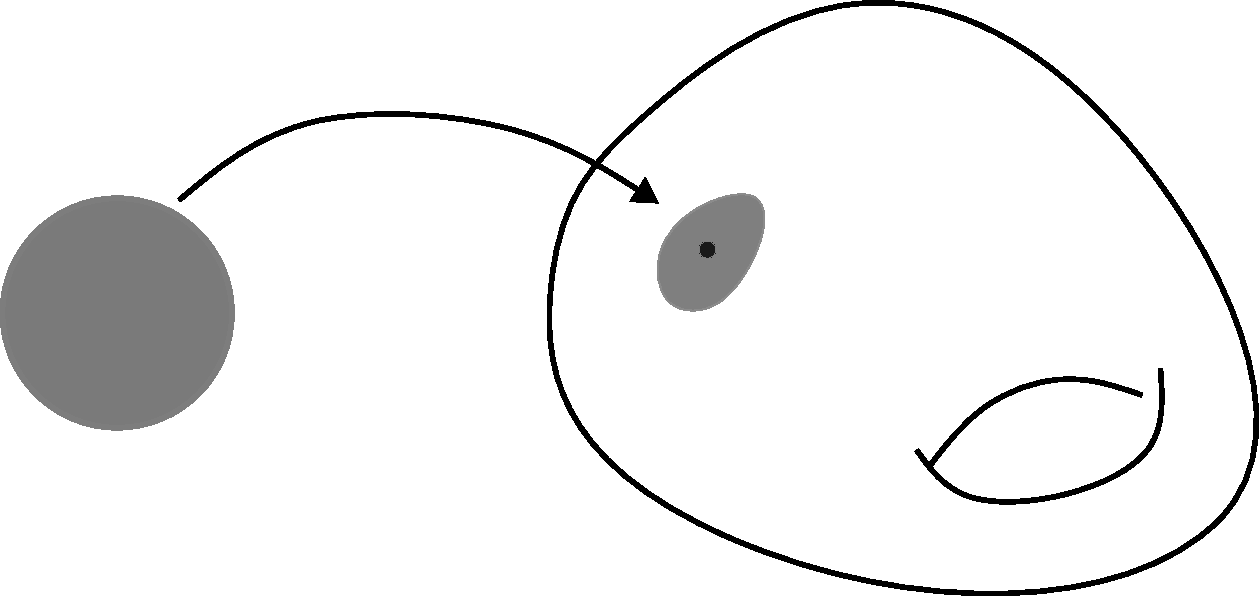
\includegraphics[width=.5\textwidth]{images/surface-parameter}
\caption{A parameterization of a neighborhood around a point on a surface.}
\label{fig:parameterization}
\end{figure}

A \EMPH{tangent vector} to $S$ at $p$ is a map $\sigma:(-\epsilon,\epsilon)\to S$ with $\sigma(0)=p$.
The set of all tangent vectors is the \EMPH{tangent plane}.
By choosing two linearly independent paths through $p\in S$ we obtain a basis 
for the tangent
plane. Using the tangent plane, we can define a normal vector $N$ at $p$.

Let
\[
X:U\subseteq\mathbb{R}^2\to\mathbb{R}^3
\]
be a smooth parameterized surface. Let $X_u$ and $X_v$
denote the partial derivatives in the directions $u$ and $v$ respectively.
 The \emph{differential} of \(X\) at
\((u,v)\in U\) is the linear map
\[
dX_{(u,v)}:T_{(u,v)}\mathbb{R}^2
\to
T_{X(u,v)}\mathbb{R}^3
\]
defined by
\[
dX_{(u,v)}(a,b)
=
aX_u(u,v)+bX_v(u,v).
\]
Similar to curves, the differential tells us how infinitesimal motions in the domain are transformed into
infinitesimal motions on the surface.
The tangent plane corresponds to the image
of the differential map $d\phi_q(\RR^2)\subset \RR^3$ (prop. 1 \cite{doc76}).

\begin{example}[The Sphere]\label{ex:sphere-charts}

We often think of the unit two sphere as a subset of $\R^3$,
the sphere is the set
$$\Sp^2=\{(x,y,z)\in \R^3 | x^2+y^2+z^2=1\}$$
We can define six charts to parameterize $\Sp^2$.
For $u,v\in[-1,1]$, we have
$$r_{z}(u,v)=(u,v,\sqrt{1-u^2-v^2}) \hspace{.5cm}  r_{-z}(u,v)=(u,v,-\sqrt{1-u^2-v^2}) \hspace{.5cm}  r_{x}(u,v)=(\sqrt{1-u^2-v^2},u,v) $$
$$r_{-x}(u,v)=(-\sqrt{1-u^2-v^2},u,v) \hspace{.5cm}  r_{y}(u,v)=(u,\sqrt{1-u^2-v^2},v) \hspace{.5cm}   r_{-y}(u,v)=(u,-\sqrt{1-u^2-v^2},v). $$

The chart $r_{z}$ is shown in \figref{sphere-chart}

\begin{figure}[htb]
	\centering
	
\includegraphics[width=.4\textwidth]{curvature/sphere-chart}
	\caption{A chart of $\Sp^2$.}
	\label{fig:sphere-chart}
\end{figure}


\end{example}

\subsection{Discrete Surfaces}

A surface can be represented by gluing together polygonal faces. The basic
building blocks of such a representation are \emph{vertices}, \emph{edges},
and \emph{faces}. We denote the sets of vertices, edges, and faces by
\(V\), \(E\), and \(F\), respectively.

A surface represented in this way is called a \emph{mesh}. If every face of
the mesh is a triangle, then it is called a \emph{triangular mesh} or
\emph{triangulated mesh}. An example of a triangular mesh is shown in
\figref{cat}. Observe that this mesh has several boundary components,
including the collar, eyes, and mouth.

Let \(\partial V\) denote the set of boundary vertices, that is, vertices
incident to the boundary of the mesh. We let \(V_{\mathrm{int}}\) denote the
set of interior vertices, namely those vertices that do not lie on the
boundary.



 \begin{figure}[htb]
         \centering
        \begin{subfigure}[b]{0.3\textwidth}
         
\includegraphics[width=\textwidth]{polygonal-mesh/profile}
         \caption{}
 	 \label{fig:profile}
       \end{subfigure}
         \hspace{.6cm}
         \begin{subfigure}[b]{0.19\textwidth}
         
\includegraphics[width=\textwidth]{polygonal-mesh/head-on}
         \caption{}
          \label{fig:head-on}
         \end{subfigure}
             \hspace{.6cm}
         \begin{subfigure}[b]{0.24\textwidth}
         
\includegraphics[width=\textwidth]{polygonal-mesh/back}
         \caption{}
          \label{fig:back}
         \end{subfigure}
		\caption{(\subref{fig:profile}) A profile view of a mesh.
 		(\subref{fig:head-on})  A frontal view of the same mesh and the view from the back (\subref{fig:back}).
 		\label{fig:cat}}
 \end{figure}
 
Examples of surface representations arise in computer graphics, 3D scanning, and the modeling of solid objects for manufacturing. When representing a smooth surface with a polygonal mesh, an important question is:
\begin{quote}
How many faces are required for the mesh to appear smooth rather than faceted?
\end{quote}
Using a larger number of smaller triangles generally produces a better approximation of the underlying surface. However, this increased accuracy comes at the cost of additional storage requirements and computational effort.

One common format for storing a mesh is the \emph{Object File Format} (OFF). The first line of an OFF file optionally identifies the file as an OFF file. The second line specifies the number of vertices, faces, and edges in the mesh. This is followed by a list of vertex coordinates in ((x,y,z))-format and a list of faces, where each face is represented by the indices of its vertices.
The OFF file corresponding to the mesh shown in \figref{cat} is given in \tabref{off}.
\small
\begin{table}[h!]
\caption{The OFF data for the mesh in \figref{cat}.}
\centering
\begin{tabular}{|p{2cm} p{2cm} p{2cm} p{2cm}|} 
 \hline
\texttt{OFF} &  & &  \\ 
\texttt{7529} & \texttt{14859} & \texttt{0} &  \\ 
\texttt{-0.29196} & \texttt{-0.0867173} & \texttt{-0.355149}  &  \\
 \texttt{-0.123586}   & \texttt{-0.0127199} & \texttt{-0.385597} &  \\
\texttt{-0.138255}   & \texttt{-0.0985078} & \texttt{-0.384018} &  \\
  & &\vdots &  \\  
 \texttt{3}&  \texttt{97} &\texttt{1893}& \texttt{1895}\\
 \texttt{3}& \texttt{71} & \texttt{1894} & \texttt{1893} \\
 \texttt{3} & \texttt{16} & \texttt{1895} & \texttt{1894}\\
   & &\vdots &  \\  
 \hline
\end{tabular}

\label{tab:off}
\end{table}
\normalsize
Suppose we work in a machine shop and a customer brings us a metal object that they would like duplicated. One approach is to create a 3D scan of the object, producing a collection of points on its surface. These points can then be used to construct a triangulated mesh representing the object, which in turn can be used to guide a computer-controlled machine in carving the object from a block of metal.

Unfortunately, errors may occur during the scanning process. As a result, the reconstructed mesh may contain self-intersections, meaning that two or more faces occupy the same region of space. If we attempt to manufacture an object from such a mesh, the machine may encounter ambiguity regarding which portions of the mesh correspond to the actual surface of the object. This motivates the development of algorithms for detecting self-intersections in meshes.

Determining whether two faces intersect directly from the OFF representation of a mesh is cumbersome. To facilitate the design of geometric algorithms, we typically convert the OFF file into a more convenient data structure known as the \emph{doubly-connected edge list} (DCEL).

The DCEL consists of three interconnected collections of objects: vertices, edges, and faces \cite{dutchbook3}. Each edge is represented by a pair of directed half-edges. For each half-edge $(\overrightarrow{e})$, we store pointers to:

\begin{itemize}
\item its origin vertex,
\item its twin half-edge,
\item the face incident to its left,
\item the next half-edge on the boundary of that face, and
\item the previous half-edge on the boundary of that face.
\end{itemize}

For each vertex (v), we store its coordinates together with a pointer to an arbitrary half-edge whose origin is (v). For each face (f), we store a pointer to an arbitrary half-edge on its boundary. If the face contains holes, we additionally store a list of inner boundary components and a pointer to a representative half-edge on the boundary of each hole.

The DCEL also provides iterators for traversing the collections of vertices, edges, and faces. Starting from an arbitrary element, these iterators allow us to visit every element in the mesh. Together, the objects and pointers maintained by the DCEL support the efficient implementation of a wide variety of geometric algorithms. A prominent example of a software library based on such data structures is the Computational Geometry Algorithms Library (CGAL) \cite{cgal,cgal:eb-24b}.

Returning to our motivating problem of detecting self-intersections, suppose a mesh (M) is stored as a DCEL. We can iterate over all pairs of faces and test whether the corresponding triangles intersect. If any pair of faces intersects, then the mesh contains a self-intersection. Pseudocode for this algorithm is given in \algref{self-intersection}.


\begin{algorithm}
 \caption{Self-intersection}\label{alg:self-intersection}
    \begin{algorithmic}[1]
      \Require A DCEL of a mesh $M.$
        \Ensure A boolean indicating if $M$ has a self-intersection.
        
        \State bool $b=0.$
\For{$f_1\in F$}
	\For{$f_2\in F$}
	
	\If{$f_1\neq f_2\ \&\&\ f_1\cap f_2 \neq \emptyset$} 
		\State $b=1.$
	\EndIf 
	\EndFor
\EndFor
\Return $b$.
\end{algorithmic}
\end{algorithm}



\subsection{The Euler Characteristic}

The \EMPH{Euler characteristic} of a surface triangulated $S$ denoted by $\chi(S)$, or $\chi$
 if the surface is clear,  is the 
the number of vertices minus the number of edges plus  the number of faces, $\chi=|V|-|E|+|F|.$
The Euler characteristic is a topological invariant of a space meaning it
and does not depend on the choice of triangulation and it is fundamental in topology
and geometry \cite{chern_triangles_1979}.
The Euler characteristic is defined for higher dimensional objects beyond surfaces,
 for a triangulated space $X$ the Euler characteristic is 
$\chi(X)=k_0-k_1+k_2-k_3+\ldots$ where $k_n$ is the number of `triangles' of dimension $n.$



A  graph  is \EMPH{planar} if it can be drawn in the plane with intersections only occurring
at vertices.
Triangulations of the two dimensional sphere $\Sp^2$ and the two dimensional disk $D^2$ 
will be used in our applications.
For the sphere, we have $\chi(\Sp^2)=2$ 
several proofs of this can be found on David Eppstein's website \cite{eppstein-proofs}.




We next give a proof that $\chi(\Sp^2)=2$ due Thurston \cite{thurston}. 
For any planar graph we imagine the graph embedded in the two sphere, by
shrinking the graph until it fits inside of the unit circle, then project the image of the graph
onto the southern hemisphere.  

\begin{theorem}[Euler Characteristic for Planar Graphs]\label{thm:euler}
For any planar graph on the two sphere we have $V-E+F=2.$
\end{theorem}

\begin{proof}
If needed, perturb the triangulation so that the north and south poles are 
inside of  two faces and there are no vertical edges. At each vertex place a unit positive
charge, at the center of each edge place a unit negative charge and put a unit positive
charge in the middle of each face. Slam the sphere on the ground so that all charges
on the edges and vertices are moved into the face below them. For faces that do not contain a pole
the net charge will be zero, the northern boundary consists of an alternating sequence
of edges and vertices  beginning  and ending with an edge.
The face containing the north pole has a unit positive charge, and the face containing the south
pole contains positive four units of charge and negative three units of charge.
Thus, the total charge is two.

\end{proof}

Triangulations of the sphere are a special case of \thmref{euler}.
The sphere will be one of two common surfaces we see in applications
of the Gauss-Bonnet theorem. The other being the disk.
For the disk, $\chi(D^2)=1$. This can be seen by considering
the removal of a single face from a triangulation of the sphere.
Once a face is removed, we can `unwrap' the remaining faces of the sphere
onto the plane to obtain a triangulation of a disk. Moreover, this projection
is invertible and given a triangulation of a disk we can obtain a triangulation
of the sphere with a single face omitted.

The Euler characteristic of a connected, orientable surface surface is often 
stated in terms of the genus of the surface which is defined as follows.
\begin{definition}[Genus of a Surface]\label{def:genus}
	The genus of a connected, orientable surface is the maximum number of
	cuttings along non-intersecting simple closed curves without disconnecting
	the surface \cite{munkres}.
\end{definition}


For an orientable surface, the genus and the Euler characteristic are related by
the formula $\chi=2-2g$. To see this, we can transform a triangulation of a surface of
genus $g$ into a surface of genus $g+1$ by removing two faces and an equal number
of vertices and edges. \figref{genus} provides an example.
Thus, the sphere has genus zero and the torus has genus one.


\begin{figure}[htb]
        \centering
        \begin{subfigure}[b]{0.2\textwidth}
        
\includegraphics[width=\textwidth]{genus/genus-1}
        \caption{Genus zero.}
          \label{fig:initial-sphere}
        \end{subfigure}
          \hspace{.5cm}
         \begin{subfigure}[b]{0.2\textwidth}
        
\includegraphics[width=\textwidth]{genus/genus-2}
        \caption{Deform.}
        \label{fig:decending-faces}
        \end{subfigure}
          \hspace{.5cm}
         \begin{subfigure}[b]{0.2\textwidth}
        
\includegraphics[width=\textwidth]{genus/genus-3}
        \caption{Triangles join.}
        \label{fig:faces-join}
        \end{subfigure}
		\caption{(\subref{fig:initial-sphere}) A surface homeomorphic to the sphere with genus zero.
		(\subref{fig:decending-faces}) The triangle on the top and the triangle on the bottom are getting
		closer. (\subref{fig:faces-join})  A surface homeomorphic to the torus. The triangle on the top
		and the triangle on the bottom have been removed. Three vertices and three edges are				removed. The Euler characteristic decreased by two.
		\label{fig:genus}}
\end{figure}



Imagine covering a surface with an arbitrary collection of open patches.
The surface is \emph{compact}, if no matter how many patches you start with, there is always a finite number of them that still cover the entire surface.
Compactness is a topological invariant. 
Every compact surface is able to be triangulated. This fact may seem intuitive but it is subtle to prove
rigorously. 

\noindent \textbf{Exercises}


\begin{enumerate}
        \item Compute the tangent plane to the sphere at the north pole.

	\item Given a mesh stored in a DCEL, give an pseudocode for an algorithm to iterate over all edges incident to a given vertex.

	
	\item How would you determine if two faces in a mesh intersect? Based on this, what is the runtime of \algref{self-intersection}?
	
	
\end{enumerate}

\pagebreak